\chapter{Designing the Data-Collection FSM (The Dataset We Can Trust)}
\label{ch:data-collection}

\section{Why a “data-collection FSM” at all?}
Chapter 2 argued that FSMs give us clarity, testability, and instrumentation---especially the power to
log clean datasets from a process that involves randomness. \cite{fsm_superpowers}
That last one (instrumentation) is our focus now: we are going to define \emph{exactly} what we log, when we log it,
and how those logs roll up into results.

This chapter produces two deliverables:
\begin{enumerate}
  \item A precise list of \textbf{fields} that define one Monty Hall trial (our row in a CSV).
  \item A \textbf{Data-Collection FSM} that tells us what happens in what order, including logging and stopping rules.
\end{enumerate}

\section{The per-trial log (one row per game)}
We will record one row per simulated trial. These are the minimum fields that let us verify randomness,
debug mistakes, and compute meaningful statistics.

\begin{table}[!ht]
\centering
\caption{Trial log fields (one row per simulated game).}
\label{tab:trial-fields}
\begin{tabular}{ll}
\toprule
Field & Meaning / why we care \\
\midrule
trial\_id & Unique integer for traceability and reproducibility \\
seed & RNG seed (optional) to reproduce a suspicious run \\
prize\_door & Where the prize was placed (should be uniform over \{1,2,3\}) \\
player\_door & The player’s initial choice (should be uniform over \{1,2,3\}) \\
reveal\_door & Host’s revealed goat door (must not equal prize\_door or player\_door) \\
decision & \texttt{stay} or \texttt{switch} (coin toss in our baseline simulation) \\
final\_door & The door the player ends on after decision \\
win & \texttt{1} if final\_door == prize\_door, else \texttt{0} \\
strategy & \texttt{random}, \texttt{always\_stay}, \texttt{always\_switch} (for experiments) \\
\bottomrule
\end{tabular}
\end{table}

\section{What we aggregate as we go (running totals)}
In addition to the per-trial log, we maintain running counters so we can:
(1) print progress, (2) build plots efficiently, and (3) decide when we have enough trials.

At minimum, keep these four “outcome buckets”:
\begin{itemize}
  \item stay\_win
  \item stay\_lose
  \item switch\_win
  \item switch\_lose
\end{itemize}

Also keep distribution checks:
\begin{itemize}
  \item counts of prize\_door = 1,2,3
  \item counts of player\_door = 1,2,3
  \item counts of decision stay vs switch
\end{itemize}

These sanity checks catch mistakes like “door 3 never gets the prize” or “my random choice is biased.”

\section{When do we stop? (confidence, not vibes)}
We want students to see the difference between:
\begin{quote}
\emph{“We ran a bunch of trials.”} \quad vs \quad \emph{“We ran enough trials to support a claim.”}
\end{quote}

We will use a confidence interval on a proportion (win-rate). Let $\hat{p}$ be the observed win-rate for a strategy,
based on $n$ trials. A simple (approximate) margin of error is:
\[
  \mathrm{halfwidth} = z \sqrt{\frac{\hat{p}(1-\hat{p})}{n}}
\]
where $z$ matches the confidence level (e.g., 1.96 for 95\%, 2.576 for 99\%). \cite{nist_ci_proportion}

\subsection{A practical stopping rule}
Pick:
\begin{itemize}
  \item confidence level (90\%, 95\%, or 99\%),
  \item a tolerance $\epsilon$ (example: $\epsilon = 0.01$ means \(\pm 1\%\)).
\end{itemize}

Stop when \textbf{both} strategy win-rates have halfwidth $\le \epsilon$:
\begin{itemize}
  \item halfwidth(switch win-rate) $\le \epsilon$
  \item halfwidth(stay win-rate) $\le \epsilon$
\end{itemize}

This makes the simulation self-aware: it runs until the estimates are sharp enough to be worth graphing.

\subsection{Worst-case “how many trials might we need?”}
Because $\hat{p}(1-\hat{p})$ is maximized at $\hat{p}=0.5$, a conservative bound is:
\[
  n \ge \frac{z^2}{4\epsilon^2}
\]
So for 99\% confidence ($z \approx 2.576$) and $\epsilon = 0.01$:
\[
  n \gtrsim \frac{(2.576)^2}{4(0.01)^2} \approx 16588
\]
That number is large on purpose: it teaches why “a few hundred trials” can still be noisy.

\section{The Data-Collection FSM (EFSM style)}
In Chapter 2 we noted that when we track extra variables like “prize door” and “player choice,”
we are really building an \emph{extended} finite state machine (EFSM). :contentReference[oaicite:3]{index=3}
Our Data-Collection FSM keeps the same clean state backbone, but annotates each step with:
\begin{itemize}
  \item which variables are set (prize\_door, player\_door, etc.)
  \item what gets logged at that step
  \item what gets aggregated
\end{itemize}

\begin{figure}[!ht]
  \centering
  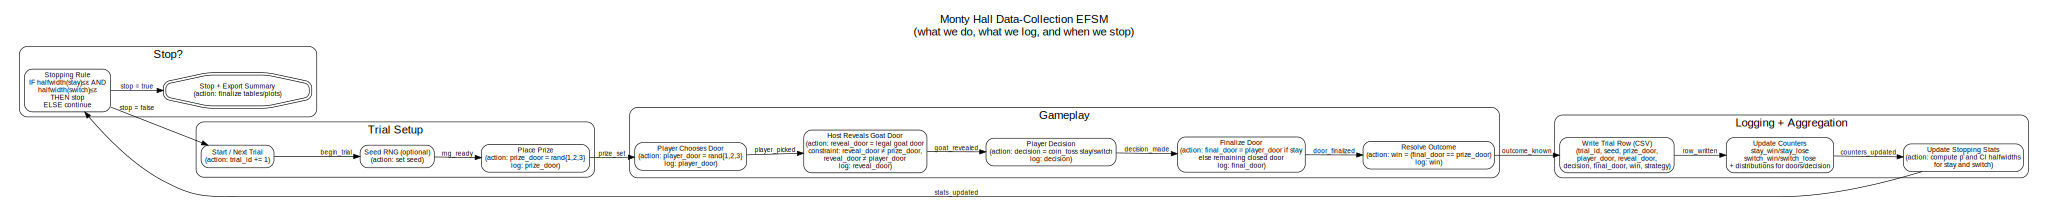
\includegraphics[width=\linewidth]{data_collection_fsm.pdf}
  \caption{Data-Collection FSM for Monty Hall simulation (Graphviz-generated).}
  \label{fig:data-collection-fsm}
\end{figure}

\section{How this maps to code (preview of Chapter 4)}
Your Chapter 2 “FSM-to-code” recipe still applies: state enum, events, transition function,
and actions on transitions. :contentReference[oaicite:4]{index=4}
The only difference is that our actions now include:
\begin{itemize}
  \item writing a trial row to CSV,
  \item updating running counters,
  \item computing confidence halfwidths and deciding whether to stop.
\end{itemize}

That is why we designed this chapter before coding: the FSM becomes the contract for both
the implementation and the unit tests.

